\documentclass{standalone}
\usepackage{../../../../preamble_tikz}

\begin{document}
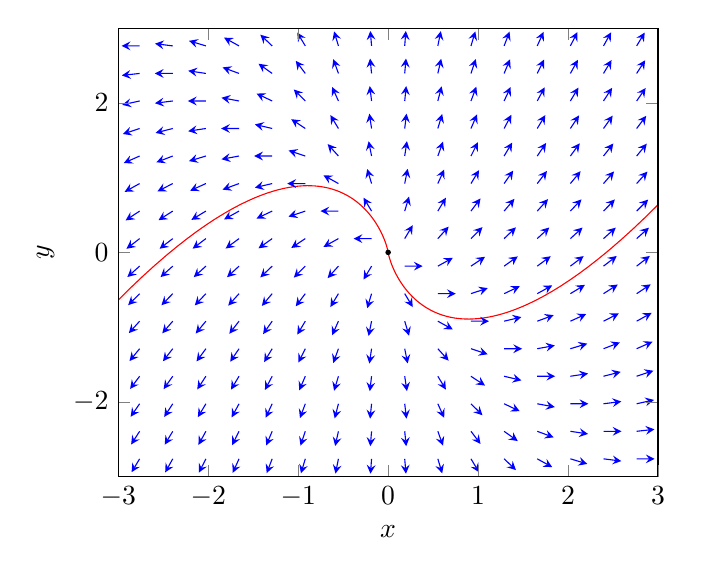
\begin{tikzpicture}
  \begin{axis}[
      xmin = -3, xmax = 3,
      ymin = -3, ymax = 3,
      zmin = 0, zmax = 1,
      xlabel = {$x$},
      ylabel = {$y$},
      view = {0}{90},
    ]
    \addplot3 [red,domain=-10:0.02,samples y=1,samples=200] ({4*exp(x)},{exp(x)*(2+4*x)},0);
    \addplot3 [red,domain=-10:0.02,samples y=1,samples=200] ({-4*exp(x)},{exp(x)*(-2-4*x)},0);
    \addplot3[
      blue,
      quiver = {
          u = {x/sqrt(x^2+(x+y)^2)},
          v = {(x+y)/sqrt(x^2+(x+y)^2)},
          scale arrows = 0.2,
        },
      -stealth,
      samples=20,
      domain = -3.5:3.5,
      domain y = -3.5:3.5,
    ] {0};
    \node[circle,fill=black,inner sep=0pt,minimum height=2pt] at (0,0){};
  \end{axis}
\end{tikzpicture}

\end{document}